\documentclass{beamer}
\usepackage{amsmath}
\usepackage[english]{babel} %set language; note: after changing this, you need to delete all auxiliary files to recompile
\usepackage[utf8]{inputenc} %define file encoding; latin1 is the other often used option
\usepackage{csquotes} % provides context sensitive quotation facilities
\usepackage{graphicx} %allows for inserting figures
\usepackage{booktabs} % for table formatting without vertical lines
\usepackage{textcomp} % allow for example using the Euro sign with \texteuro
\usepackage{stackengine}
\usepackage{wasysym}
\usepackage{tikzsymbols}
\usepackage{textcomp}
\newcommand{\bubblethis}[2]{
        \tikz[remember picture,baseline]{\node[anchor=base,inner sep=0,outer sep=0]%
        (#1) {\underline{#1}};\node[overlay,cloud callout,callout relative pointer={(0.2cm,-0.7cm)},%
        aspect=2.5,fill=yellow!90] at ($(#1.north)+(-0.5cm,1.6cm)$) {#2};}%
    }%
\tikzset{face/.style={shape=circle,minimum size=4ex,shading=radial,outer sep=0pt,
        inner color=white!50!yellow,outer color= yellow!70!orange}}
%% Some commands to make the code easier
\newcommand{\emoticon}[1][]{%
  \node[face,#1] (emoticon) {};
  %% The eyes are fixed.
  \draw[fill=white] (-1ex,0ex) ..controls (-0.5ex,0.2ex)and(0.5ex,0.2ex)..
        (1ex,0.0ex) ..controls ( 1.5ex,1.5ex)and( 0.2ex,1.7ex)..
        (0ex,0.4ex) ..controls (-0.2ex,1.7ex)and(-1.5ex,1.5ex)..
        (-1ex,0ex)--cycle;}
\newcommand{\pupils}{
  %% standard pupils
  \fill[shift={(0.5ex,0.5ex)},rotate=80] 
       (0,0) ellipse (0.3ex and 0.15ex);
  \fill[shift={(-0.5ex,0.5ex)},rotate=100] 
       (0,0) ellipse (0.3ex and 0.15ex);}

\newcommand{\emoticonname}[1]{
  \node[below=1ex of emoticon,font=\footnotesize,
        minimum width=4cm]{#1};}
\usepackage{scalerel}
\usetikzlibrary{positioning}
\usepackage{xcolor,amssymb}
\newcommand\dangersignb[1][2ex]{%
  \scaleto{\stackengine{0.3pt}{\scalebox{1.1}[.9]{%
  \color{red}$\blacktriangle$}}{\tiny\bfseries !}{O}{c}{F}{F}{L}}{#1}%
}
\newcommand\dangersignw[1][2ex]{%
  \scaleto{\stackengine{0.3pt}{\scalebox{1.1}[.9]{%
  \color{red}$\blacktriangle$}}{\color{white}\tiny\bfseries !}{O}{c}{F}{F}{L}}{#1}%
}
\usepackage{fontawesome} % Social Icons
\usepackage{epstopdf} % allow embedding eps-figures
\usepackage{tikz} % allows drawing figures
\usepackage{amsmath,amssymb,amsthm} %advanced math facilities
\usepackage{lmodern} %uses font that support italic and bold at the same time
\usepackage{tikz}
\usepackage{tcolorbox}

\usefonttheme[onlymath]{serif} %set math font to serif ones

\definecolor{beamerblue}{rgb}{0.2,0.2,0.7} %define beamerblue color for later use

%%% defines highlight command to set text blue
\newcommand{\highlight}[1]{{\color{blue}{#1}}}


%%%%%%% commands defining backup slides so that frame numbering is correct

\newcommand{\backupbegin}{
   \newcounter{framenumberappendix}
   \setcounter{framenumberappendix}{\value{framenumber}}
}
\newcommand{\backupend}{
   \addtocounter{framenumberappendix}{-\value{framenumber}}
   \addtocounter{framenumber}{\value{framenumberappendix}}
}

%%%% end of defining backup slides

%Specify figure caption, see also http://tex.stackexchange.com/questions/155738/caption-package-not-working-with-beamer
\setbeamertemplate{caption}{\insertcaption} %redefines caption to remove label "Figure".
%\setbeamerfont{caption}{size=\scriptsize,shape=\itshape,series=\bfseries} %sets figure  caption bold and italic and makes it smaller


\usetheme{Boadilla}

% --------------------
% Overall information
% --------------------
\title[Economía I]{Economía I \vspace{4mm}
\\ Magistral 25: Politica fiscal}
\date{}
\author[Riottini]{Riottini Franco}
\vspace{0.4cm}
\institute[]{Universidad de San Andrés} 


\begin{document}

\begin{frame}
\titlepage
\centering
Magistral 26

\includegraphics[scale=0.2]{../Figures/logoUDESA.jpg} 
\end{frame}

\begin{frame}{}
\centering 	\huge \textbf{Política fiscal} 
\vspace{2mm}
\hrule
\end{frame}


\begin{frame}{¿Cómo funciona la política fiscal?}
    \begin{itemize}
        \item El análisis de la política fiscal es mucho más complejo por una serie de motivos:
        \begin{itemize}
            \item La política fiscal expansiva genera aumentos de la demanda agregada 
            \item Pero la política fiscal requiere financiamiento
            \begin{itemize}
                \item Necesitamos entender cómo puede financiar el Gobierno para hacer uso de este instrumento
            \end{itemize}
            \item Hay efectos expulsión (“crowding out”) vía la tasa de interés (que no aparecían con la política monetaria)
        \end{itemize}
        \vspace{2mm}
        \item La combinación de estos tres factores nos dará el efecto neto de la política fiscal sobre la demanda agregada
    \end{itemize}
\end{frame}

\begin{frame}{¿Cómo puede financiar el gasto un gobierno?}
    \begin{itemize}
        \item Existen cuatro mecanismos básicos para financiar la política fiscal:
        \begin{itemize}
            \item Hacer emisión monetaria 
            \item Aumentar los impuestos
            \item Pedir deuda
        \end{itemize}
        \vspace{2mm}
        \item Cada uno de estos implicará distintos mecanismos sobre la demanda agregada
    \end{itemize}
\end{frame}


\begin{frame}{El efecto “financiamiento” sobre el consumo: impuestos}
    
    \begin{itemize}
        \item Si aumenta el gasto público financiado enteramente con impuestos: ¿cuánto cae el consumo privado?
        \begin{itemize}
            \item Cae el consumo que esos impuestos desplazan
            \item Si los impuestos son permanentes la caída del consumo debiera ser el 100\% del aumento de los impuestos (primer caso)
            \item La caída del consumo es menor si se piensa que es transitorio y podría aumentar el producto en le corto plazo (segundo y tercer caso)
            \item Lo cierto es que el efecto de la política fiscal se modera sustancialmente cuando se tiene en cuenta el financiamiento
        \end{itemize}
        \end{itemize}

\end{frame}

% \begin{frame}{¿Cuándo tiene, entonces, la política fiscal un efecto sobre la demanda agregada?}

%     \begin{itemize}
%     \item Cuando no hay una reducción equivalente del consumo privado
%     \end{itemize}
%      \vspace{3mm}
    
%     \centering\includegraphics[width=6cm]{../P95b.png}\

% \end{frame}

%---------------------------------------------------------------------------%

\begin{frame}{Expansión fiscal c/impuestos (permanentes/clásico)}
   
 \begin{center}
\begin{figure}[H]
\renewcommand{\figurename}{Figure}
\begin{center}
    \begin{minipage}[b]{0.45\textwidth}
        \begin{center}
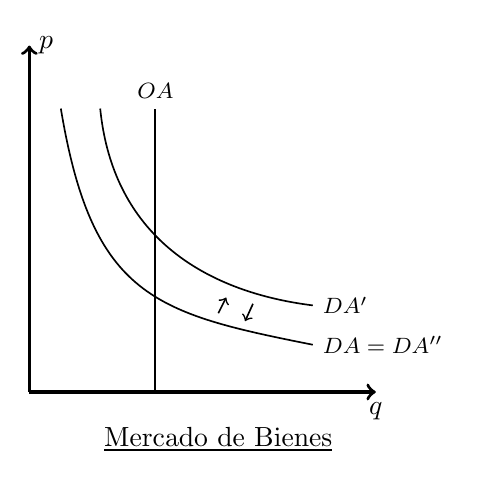
\begin{tikzpicture}[scale=0.4]
\draw[very thick,<-] (0,11)--(0,0);
\draw[very thick,->] (0,0)--(11,0) node[below]{$q$};
\node[right] at (0,11) {$p$};

\node[] at(6,-1.5) {\underline{Mercado de Bienes}};
\draw[semithick] (1,9).. controls (2,3) and (4, 2.5) .. (9, 1.5) node [right]{\footnotesize $DA=DA''$};
\draw[semithick] (2.25,9).. controls (2.75,4) and (7, 3) .. (9, 2.75) node [right]{\footnotesize $DA'$};
\draw[semithick](4, 0)--(4, 9) node [above]{\footnotesize $OA$};
\draw[semithick, ->] (6,2.5)--(6.25,3);
\draw[semithick, <-] (6.85,2.25)--(7.1,2.8);
%\draw[thick, gray, dashed] (4,3)--(0,3);
\end{tikzpicture}
\end{center}
     \end{minipage}
  %  \hfill
    \begin{minipage}[b]{0.45\textwidth}
    \begin{center}
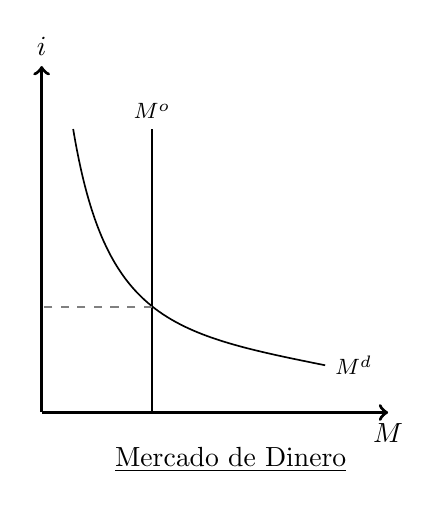
\begin{tikzpicture}[scale=0.4]
\draw[very thick,<-] (0,11) node[above]{$i$}--(0,0);
\draw[very thick,->] (0,0)--(11,0) node[below]{$M$};
\node[right] at (0,11) {};

\node[] at(6,-1.5) {\underline{Mercado de Dinero}};
\draw[semithick] (1,9).. controls (2,3) and (4, 2.5) .. (9, 1.5) node [right]{\footnotesize $M^{d}$};
\draw[semithick](3.5, 0)--(3.5, 9) node [above]{\footnotesize $M^{o}$};

 \draw[thick, gray, dashed] (3.5,3.35)--(0,3.35);

\end{tikzpicture}
\end{center}
    \end{minipage}
\end{center}
\vspace{0.7cm}
\label{fig:C36.2}
\end{figure}
\end{center}   
   
\end{frame}

\begin{frame}{Expansión fiscal c/impuestos (permanentes/keynesiano)}
\begin{center}
\begin{figure}[H]
\renewcommand{\figurename}{Figure}
\begin{center}
    \begin{minipage}[b]{0.45\textwidth}
        \begin{center}
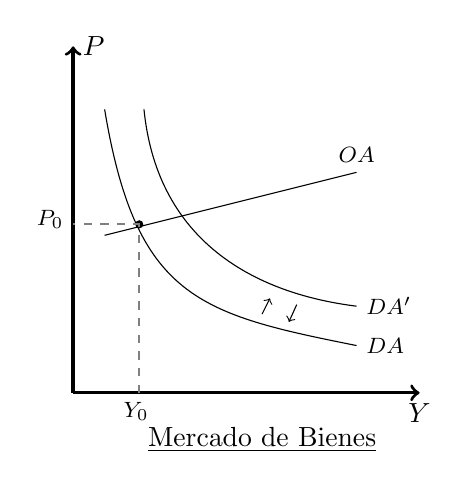
\begin{tikzpicture}[scale=0.4]
\draw[very thick,<-] (0,11)--(0,0);
\draw[very thick,->] (0,0)--(11,0) node[below]{$Y$};
\node[right] at (0,11) {$P$};

\node[] at(6,-1.5) {\underline{Mercado de Bienes}};
\draw[thin] (1,9).. controls (2,3) and (4, 2.5) .. (9, 1.5) node [right]{\footnotesize $DA$};
\draw[thin] (2.25,9).. controls (2.75,4) and (7, 3) .. (9, 2.75) node [right]{\footnotesize $DA'$};
\draw[thin](1, 5)--(9,7) node [above]{\footnotesize $OA$};
\draw[thin, ->] (6,2.5)--(6.25,3);
\draw[thin, <-] (6.85,2.25)--(7.1,2.8);
\node[below] at (2,0) {\footnotesize $Y_0$};
\node[left] at (0,5.5) {\footnotesize $P_0$};
\draw[fill] (2.1,5.35) circle [radius =0.11];
 \draw[thick, gray, dashed] (2.1,0)--(2.1,5.35)--(0,5.35);

\end{tikzpicture}
\end{center}
     \end{minipage}
  %  \hfill
    \begin{minipage}[b]{0.45\textwidth}
    \begin{center}
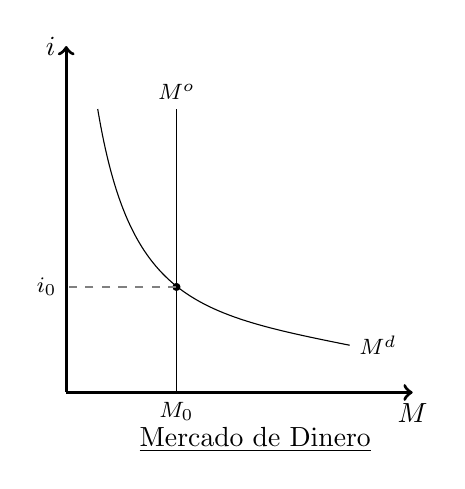
\begin{tikzpicture}[scale=0.4]
\draw[very thick,<-] (0,11) node[left]{$i$}--(0,0);
\draw[very thick,->] (0,0)--(11,0) node[below]{$M$};
\node[right] at (0,11) {};

\node[] at(6,-1.5) {\underline{Mercado de Dinero}};
\draw[thin] (1,9).. controls (2,3) and (4, 2.5) .. (9, 1.5) node [right]{\footnotesize $M^{d}$};
\draw[thin](3.5, 0)--(3.5, 9) node [above]{\footnotesize $M^{o}$};
\node[below] at (3.5,0) {\footnotesize $M_0$};
\node[left] at (0,3.35) {\footnotesize $i_0$};
\draw[fill] (3.5,3.35) circle [radius =0.11];
\draw[thick, gray, dashed] (3.5,3.35)--(0,3.35);

\end{tikzpicture}
\end{center}
    \end{minipage}
\end{center}
\end{figure}
\end{center} 
\end{frame}

\begin{frame}{Expansión fiscal con impuestos permanentes}
   Conclusiones:
   \begin{itemize}
       \item No hay efectos: lo que el gobierno gasta, la gente lo deja de gastar.
       \item La demanda agregada no se modifica
       \item No importa como es la curva de oferta
       \item Es decir el resultado es el mismo en el mundo clásico o keynesiano
   \end{itemize}
\end{frame}


\begin{frame}{Expansión fiscal c/ impuestos transitorios/clásico}
\begin{center}
\begin{figure}[H]
\renewcommand{\figurename}{Figure}
\begin{center}
    \begin{minipage}[b]{0.45\textwidth}
        \begin{center}
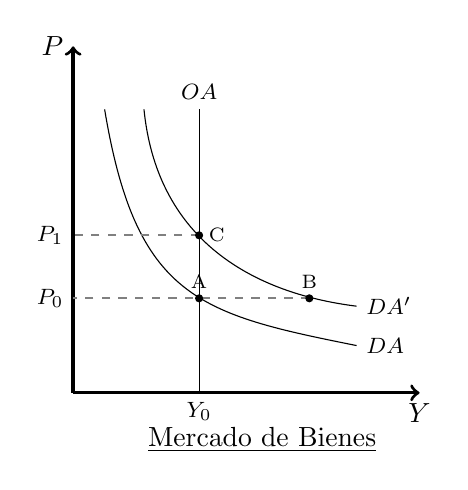
\begin{tikzpicture}[scale=0.4]
\draw[very thick,<-] (0,11)--(0,0);
\draw[very thick,->] (0,0)--(11,0) node[below]{$Y$};
\node[left] at (0,11) {$P$};
\node[] at(6,-1.5) {\underline{Mercado de Bienes}};
\draw[thin] (1,9).. controls (2,3) and (4, 2.5) .. (9, 1.5) node [right]{\footnotesize $DA$};
\draw[thin] (2.25,9).. controls (2.75,4) and (7, 3) .. (9, 2.75) node [right]{\footnotesize $DA'$};
\draw[thin](4, 0)--(4, 9) node [above]{\footnotesize $OA$};
\draw[thick, gray, dashed] (7.5,3)--(0,3);
\draw[thick, gray, dashed] (4,5)--(0,5);
\draw[fill] (7.5,3) circle [radius =0.11] node[above] {\scriptsize B};
\draw[fill] (4,5) circle [radius =0.11] node[right] {\scriptsize C};
\node[below] at (4,0) {\footnotesize $Y_0$};
\node[left] at (0,3) {\footnotesize $P_0$};
\node[left] at (0,5) {\footnotesize $P_1$};
\draw[fill] (4,3) circle [radius =0.11] circle [radius =0.11] node[above] {\scriptsize A};
%\draw[thick, gray, dashed] (2.1,0)--(2.1,5.35)--(0,5.35);
\end{tikzpicture}
\end{center}
     \end{minipage}
  %  \hfill
    \begin{minipage}[b]{0.45\textwidth}
    \begin{center}
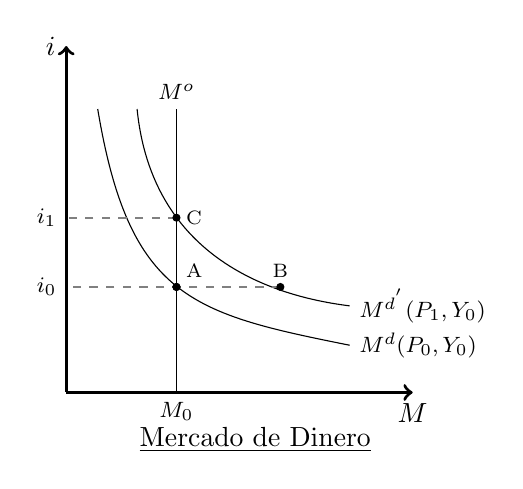
\begin{tikzpicture}[scale=0.4]
\draw[very thick,<-] (0,11) node[left]{$i$}--(0,0);
\draw[very thick,->] (0,0)--(11,0) node[below]{$M$};
\node[right] at (0,11) {};
\node[] at(6,-1.5) {\underline{Mercado de Dinero}};
\draw[thin] (1,9).. controls (2,3) and (4, 2.5) .. (9, 1.5) node [right]{\footnotesize $M^{d} (P_0, Y_0)$};
\draw[thin] (2.25,9).. controls (2.75,4) and (7, 3) .. (9, 2.75) node [right]{\footnotesize $M^{d^{'}} (P_1, Y_0)$};
\draw[thin](3.5, 0)--(3.5, 9) node [above]{\footnotesize $M^{o}$};
 \draw[thick, gray, dashed] (6.8,3.35)--(0,3.35);
 \draw[thick, gray, dashed] (3.5,5.55)--(0,5.55);
 %\draw[thin, ->] (6,2.5)--(6.25,3);
%\draw[thin, <-] (6.85,2.25)--(7.1,2.8);
\draw[fill] (3.5,3.35) circle [radius =0.11] node[above right] {\scriptsize A};
\draw[fill] (6.8,3.35) circle [radius =0.11] node[above] {\scriptsize B};
\draw[fill] (3.5,5.55) circle [radius =0.11] node[right] {\scriptsize C};
\node[below] at (3.5,0) {\footnotesize $M_0$};
\node[left] at (0,3.35) {\footnotesize $i_0$};
\node[left] at (0,5.55) {\footnotesize $i_1$};
\draw[fill] (3.5,3.35) circle [radius =0.11];
\end{tikzpicture}
\end{center}
    \end{minipage}
\end{center}
\end{figure}
\end{center} 
\end{frame}

%---------------------------------------------------------------------------%
\begin{frame}{Expansión fiscal c/impuestos transitorios/clásico}
   
\begin{itemize}
    \item La reversión de la demanda agregada no es plena
    \item El exceso de demanda empuja los precios para arriba
    \item Eso aumenta la demanda de dinero empujando para arriba la tasa de interés 
    \item A la postre el crowding out es pleno
    \end{itemize}
\end{frame}

%---------------------------------------------------------------------------%
\begin{frame}{Expansión fiscal c/impuestos transitorios/keynesiano}
\begin{center}
\begin{figure}[H]
\renewcommand{\figurename}{Figure}
\begin{center}
\begin{minipage}[b]{0.45\textwidth}
\begin{center}
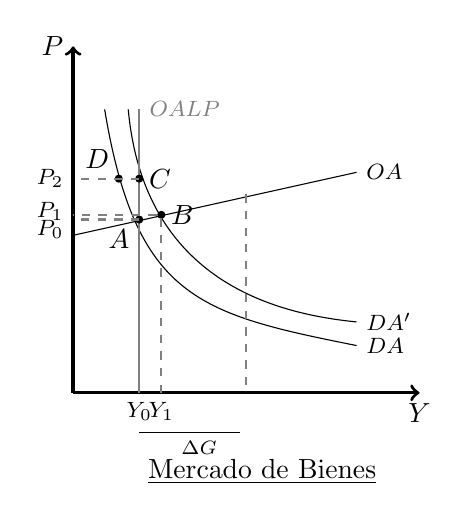
\begin{tikzpicture}[scale=0.4]
\draw[very thick,<-] (0,11)--(0,0);
\draw[very thick,->] (0,0)--(11,0) node[below]{$Y$};
\node[left] at (0,11) {$P$};

\node[] at(6,-2.5) {\underline{Mercado de Bienes}};
\draw[thin] (1,9).. controls (2,3) and (4, 2.5) .. (9, 1.5) node [right]{\footnotesize $DA$};
\draw[thin] (1.75,9).. controls (2.25,3.5) and (6.5,2.5) .. (9, 2.25) node [right]{\footnotesize $DA'$};
\draw[thin](0, 5)--(9, 7) node [right]{\footnotesize $OA$};
\draw [thin](2.1,-1.25) -- (5.3,-1.25);
\draw (4,-1.75) node[]{\scriptsize $\Delta G $};
\draw[thick, gray] (2.1,0)--(2.1,9) node [right]{\footnotesize $OALP$};;
\draw[thick, gray, dashed] (5.5,6.3)--(5.5,0);
\draw[fill] (2.1,5.5) circle [radius =0.11] node[below left] {$A$}; 
\draw[fill] (2.8,5.65) circle [radius =0.11] node[right] {$B$}; 
\draw[fill] (2.1,6.8) circle [radius =0.11] node[right] {$C$}; 
\draw[fill] (1.45,6.8) circle [radius =0.11] node[above left] {$D$}; 
\node[below] at (2.1,0) {\footnotesize $Y_0$};
\node[below] at (2.8,0) {\footnotesize $Y_1$};
\node[left] at (0,5.2) {\footnotesize $P_0$};
\node[left] at (0,5.75) {\footnotesize $P_1$};
\node[left] at (0,6.8) {\footnotesize $P_2$};
\draw[thick, gray, dashed] (2.1,6.8)--(0,6.8);
\draw[thick, gray, dashed] (2.8,0)--(2.8,5.65)--(0,5.65);
\draw[thick, gray, dashed] (2.1,5.5)--(0,5.5);
\end{tikzpicture}
\end{center}
\end{minipage}
\begin{minipage}[b]{0.45\textwidth}
\begin{center}
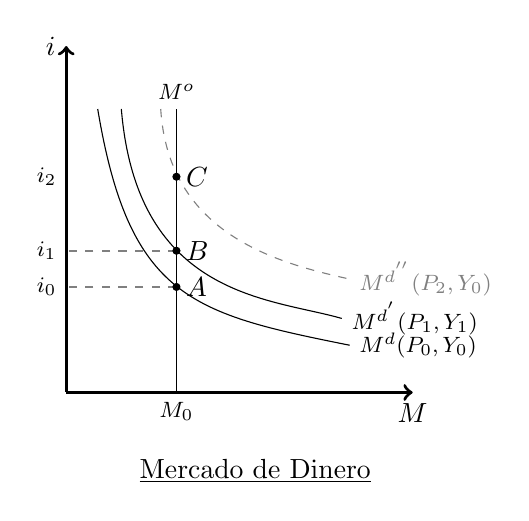
\begin{tikzpicture}[scale=0.4]
\draw[very thick,<-] (0,11) node[left]{$i$}--(0,0);
\draw[very thick,->] (0,0)--(11,0) node[below]{$M$};
\node[right] at (0,11) {};
\node[] at(6,-2.5) {\underline{Mercado de Dinero}};
\draw[thin] (1,9).. controls (2,3) and (4, 2.5) .. (9, 1.5) node [right]{\footnotesize $M^{d} (P_0, Y_0)$};
\draw[thin] (1.75,9).. controls (2.25,3) and (6.5, 3) .. (8.75, 2.35) node [right]{\footnotesize $M^{d^{'}} (P_1, Y_1)$};
\draw[thin, gray, dashed] (3,9).. controls (3.25,5) and (6.75,4.1) .. (9,3.6) node [right]{\footnotesize $M^{d^{''}} (P_2, Y_0)$};
\draw[thin](3.5, 0)--(3.5, 9) node [above]{\footnotesize $M^{o}$};
\draw[thick, gray, dashed] (3.5,3.35)--(0,3.35);
\draw[thick, gray, dashed] (3.5,4.5)--(0,4.5);
\draw[fill] (3.5,3.35) circle [radius =0.11] node[right] {$A$}; 
\draw[fill] (3.5,4.5) circle [radius =0.11] node[right] {$B$}; 
\draw[fill] (3.5,6.85) circle [radius =0.11] node[right] {$C$};
\node[below] at (3.5,0) {\footnotesize $M_0$};
\node[left] at (0,3.35) {\footnotesize $i_0$};
\node[left] at (0,4.5) {\footnotesize $i_1$};
\node[left] at (0,6.85) {\footnotesize $i_2$};
\end{tikzpicture}
\end{center}
\end{minipage}
\end{center}
\end{figure}
\end{center} 
\end{frame}

\begin{frame}{Expansión fiscal c/impuestos transitorios/keynesiano}
   
\begin{itemize}
    \item La reversión de la demanda agregada no es plena
    \item El exceso de demanda hace subir el producto 
    \item Eso aumenta la demanda de dinero empujando para arriba la tasa de interés 
    \item La tasa de interés sube menos (que en el caso clásico) y el producto se expande 
    \item Los precios empiezan  a subir, cuando la politica se revierte, se pasa por una fase recesiva 
\end{itemize}
    
\end{frame}


%---------------------------------------------------------------------------%


\begin{frame}{¿Cómo funciona la política fiscal financiada con deuda?}

    \begin{itemize}
    \item Acá el punto clave es si los agentes anticipan la carga impositiva que implica la mayor deuda
    \item Si se anticipan los impuestos necesarios para pagar esta deuda, es igual que el caso anterior (equivalencia ricardiana)
    \item En la práctica se encuentra que el ahorro responde a la deuda, pero que la compensación no es plena
    \item En tanto el efecto no es de compensación plena, hay un efecto expansivo en la demanda agregada (con efecto sobre el producto en un mundo keynesiano)

    \end{itemize}

\end{frame}


\begin{frame}{El efecto “financiamiento” sobre el consumo: deuda }
    
    \begin{itemize}
        \item Si aumenta el gasto público financiado con deuda: ¿cuánto cae el consumo privado?
        \begin{itemize}
            \item En principio podríamos pensar que nada 
            \item Pero si existe “equivalencia ricardiana”, cae igual que si se financia con impuestos (casos anteriores)
            \item Y hay crowding out también si hay un aumento en la tasa de interés 
        \end{itemize}
    \end{itemize}

\end{frame}
%---------------------------------------------------------------------------%

\begin{frame}{Ejemplo de equivalencia ricardiana}
    
\begin{itemize}
    \item Supongamos dos periodos en los que el individuo tiene ingresos de 1000 y 1000
    \item El gobierno quiere gastar 100 y 100 
    \item Lo financia con deuda en el primer periodo y la tasa de interés es 10\%
    \item El agente enfrenta impuestos de 0 y 210
    \item Si consume su ingreso consumiría 1000 y 790 
    \item ¿Qué pasa si ahorra 100 en el primero período?
    \item Ahora puede consumir 900 y 900 (que es mejor que 1000 y 790)
    \item Pero 900 y 900 ¡es lo mismo que si el gobierno hubiera financiado los 100 con impuestos! 
\end{itemize}

\end{frame}

%---------------------------------------------------------------------------%

% \begin{frame}{¿Pero existe ese fenómeno Ricardiano? I}

%      \begin{center}
%          Correlación entre deuda pública y activos financieros netos acumulados por los hogares
%      \end{center}

%      \centering\includegraphics[width=11cm]{../P91b.png}\  

%      \begin{center}
%          Grennes y Strazds (2013) en base a datos de Eurostat
%      \end{center}

% \end{frame}


% \begin{frame}{¿Pero existe ese fenómeno Ricardiano? II}
%  \centering\includegraphics[width=13cm]{../Figures/C36.11.png}\  
% \begin{itemize}
% \end{itemize}

% \end{frame}


\begin{frame}{Expansión fiscal/deuda/ricardianos/permanente}
   
 \begin{center}
\begin{figure}[H]
\renewcommand{\figurename}{Figure}
\begin{center}
    \begin{minipage}[b]{0.45\textwidth}
        \begin{center}
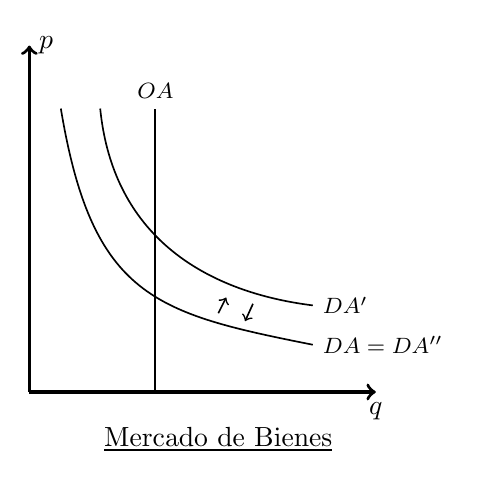
\begin{tikzpicture}[scale=0.4]
\draw[very thick,<-] (0,11)--(0,0);
\draw[very thick,->] (0,0)--(11,0) node[below]{$q$};
\node[right] at (0,11) {$p$};

\node[] at(6,-1.5) {\underline{Mercado de Bienes}};
\draw[semithick] (1,9).. controls (2,3) and (4, 2.5) .. (9, 1.5) node [right]{\footnotesize $DA=DA''$};
\draw[semithick] (2.25,9).. controls (2.75,4) and (7, 3) .. (9, 2.75) node [right]{\footnotesize $DA'$};
\draw[semithick](4, 0)--(4, 9) node [above]{\footnotesize $OA$};
\draw[semithick, ->] (6,2.5)--(6.25,3);
\draw[semithick, <-] (6.85,2.25)--(7.1,2.8);
%\draw[thick, gray, dashed] (4,3)--(0,3);
\end{tikzpicture}
\end{center}
     \end{minipage}
  %  \hfill
    \begin{minipage}[b]{0.45\textwidth}
    \begin{center}
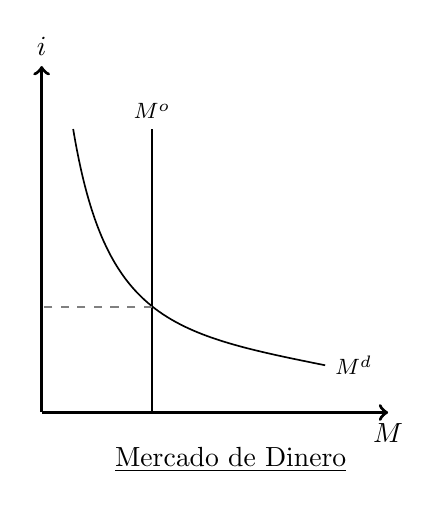
\begin{tikzpicture}[scale=0.4]
\draw[very thick,<-] (0,11) node[above]{$i$}--(0,0);
\draw[very thick,->] (0,0)--(11,0) node[below]{$M$};
\node[right] at (0,11) {};

\node[] at(6,-1.5) {\underline{Mercado de Dinero}};
\draw[semithick] (1,9).. controls (2,3) and (4, 2.5) .. (9, 1.5) node [right]{\footnotesize $M^{d}$};
\draw[semithick](3.5, 0)--(3.5, 9) node [above]{\footnotesize $M^{o}$};
 \draw[thick, gray, dashed] (3.5,3.35)--(0,3.35);
\end{tikzpicture}
\end{center}
    \end{minipage}
\end{center}
\end{figure}
\end{center}  
\end{frame}


\begin{frame}{Expansión fiscal/deuda/ricardianos/permanente}   
\begin{itemize}
\item El resultado para keynesianos o clásicos es idéntico a la política fiscal financiada con impuestos permanentes
\item La reversión de la demanda agregada es plena y no se modifica por consiguiente no tenemos efectos en el mercado monetario y de trabajo
\item En el mercado de credito aparece la demanda del gobierno
\item Pero como la gente (ricardiana) anticipa los mayores impuestos aumenta su ahorro en la misma magnitud! 
\item Con lo cual no se modifican las tasas de interés 
\item De hecho una de las pruebas de si hay equivalencia ricardiana es ver si las tasas de interés cambian con el déficit fiscal
\end{itemize}    
\end{frame}



\begin{frame}{Expansión fiscal/deuda/ricardianos/transitorio}
\begin{itemize}
\item El resultado para keynesianos o clásicos es idéntico a la política fiscal financiada con impuestos transitorios
\item Aquí, la demanda agregada se incrementa 
\item El gasto se financia con deuda, aumenta la demanda de crédito y disminuye el consumo.
\item En un contexto clásico se produce un crowding out del 100%, 
\item En el mundo keynesiano se produce una expansión del producto en el corto plazo.
\end{itemize}
\end{frame}


\begin{frame}{Expansión fiscal/deuda/no ricardianos/clasico}
\begin{center}
\begin{figure}[H]
\renewcommand{\figurename}{Figure}
\begin{center}
\begin{minipage}[b]{0.45\textwidth}
\begin{center}
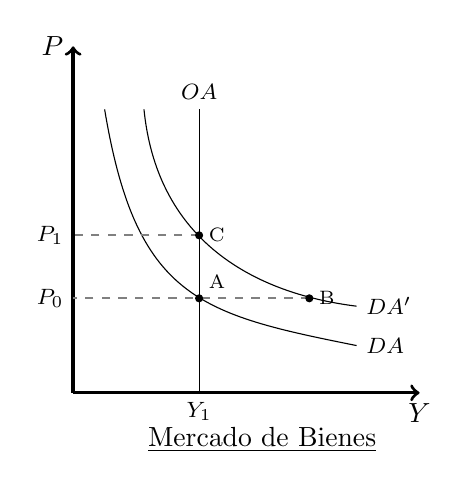
\begin{tikzpicture}[scale=0.4]
\draw[very thick,<-] (0,11)--(0,0);
\draw[very thick,->] (0,0)--(11,0) node[below]{$Y$};
\node[left] at (0,11) {$P$};
\node[] at(6,-1.5) {\underline{Mercado de Bienes}};
\draw[thin] (1,9).. controls (2,3) and (4, 2.5) .. (9, 1.5) node [right]{\footnotesize $DA$};
\draw[thin] (2.25,9).. controls (2.75,4) and (7, 3) .. (9, 2.75) node [right]{\footnotesize $DA'$};
\draw[thin](4, 0)--(4, 9) node [above]{\footnotesize $OA$};
\draw[thick, gray, dashed] (7.5,3)--(0,3);
\draw[thick, gray, dashed] (4,5)--(0,5);
\draw[fill] (4,3) circle [radius =0.11] node[above right] {\scriptsize A};
\draw[fill] (7.5,3) circle [radius =0.11] node[right] {\scriptsize B};
\draw[fill] (4,5) circle [radius =0.11] node[right] {\scriptsize C};
\node[below] at (4,0) {\footnotesize $Y_1$};
\node[left] at (0,3) {\footnotesize $P_0$};
\node[left] at (0,5) {\footnotesize $P_1$};

\end{tikzpicture}
\end{center}
\end{minipage}
\begin{minipage}[b]{0.45\textwidth}
\begin{center}
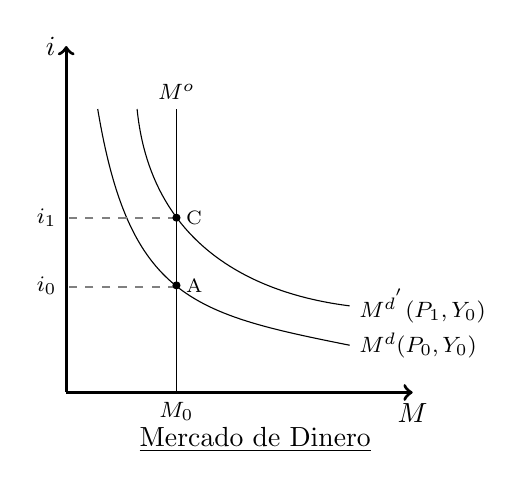
\begin{tikzpicture}[scale=0.4]
\draw[very thick,<-] (0,11) node[left]{$i$}--(0,0);
\draw[very thick,->] (0,0)--(11,0) node[below]{$M$};
\node[right] at (0,11) {};
\node[] at(6,-1.5) {\underline{Mercado de Dinero}};
\draw[thin] (1,9).. controls (2,3) and (4, 2.5) .. (9, 1.5) node [right]{\footnotesize $M^{d} (P_0, Y_0)$};;
\draw[thin] (2.25,9).. controls (2.75,4) and (7, 3) .. (9, 2.75) node [right]{\footnotesize $M^{d^{'}} (P_1, Y_0)$};
\draw[thin](3.5, 0)--(3.5, 9) node [above]{\footnotesize $M^{o}$};
\draw[thick, gray, dashed] (3.5,3.35)--(0,3.35);
\draw[thick, gray, dashed] (3.5,5.55)--(0,5.55);
\draw[fill] (3.5,3.4) circle [radius =0.11] node[right] {\scriptsize A}; 
\draw[fill] (3.5,5.55) circle [radius =0.11] node[right] {\scriptsize C};  
\node[below] at (3.5,0) {\footnotesize $M_0$};
\node[left] at (0,3.4) {\footnotesize $i_0$};
\node[left] at (0,5.55) {\footnotesize $i_1$};
\end{tikzpicture}
\end{center}
\end{minipage}
\end{center}
\end{figure}
\end{center} 
\end{frame}

\begin{frame}{Expansión fiscal/deuda/no ricardianos/clásico}
\begin{itemize}
\item La reversión de la demanda agregada no es plena con lo que aumenta 
\item Los precios aumentan eliminando el exceso de demanda
\item Esto empuja para arriba la demanda de dinero-
\item En el mercado de crédito el gobierno aumenta la demanda incrementando la tasa de interés. 
\item Como a la tasa de interés del mercado de crédito hay un exceso de oferta de dinero la tasa de interés se ubica en un valor algo menor. 
\item Pero el crowding out es total
\item Porque lo que toma el gobierno es exacto lo que tiene que caer el consumo y la inversión. 
\item En el mercado de trabajo los salarios acompañan a los precios sin efecto en el empleo 
\end{itemize}    
\end{frame}

\begin{frame}{Expansión fiscal/deuda/no ricardianos/keynesiano}
\begin{center}
\begin{figure}[H]
\renewcommand{\figurename}{Figure}
\begin{center}
\begin{minipage}[b]{0.45\textwidth}
\begin{center}
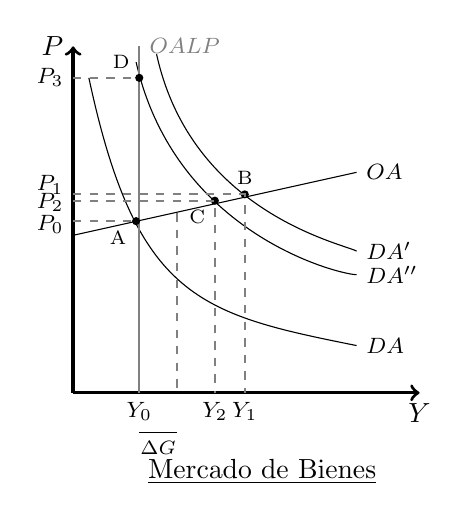
\begin{tikzpicture}[scale=0.4]
\draw[very thick,<-] (0,11)--(0,0);
\draw[very thick,->] (0,0)--(11,0) node[below]{$Y$};
\node[left] at (0,11) {$P$};
\node[] at(6,-2.5) {\underline{Mercado de Bienes}};
\draw[thin] (0.5,10).. controls (2,3) and (4, 2.5) .. (9, 1.5) node [right]{\footnotesize $DA$};
\draw[thin] (2.65,10.75).. controls (3.75,5.75) and (8.5, 4.75) .. (9, 4.5) node [right]{\footnotesize $DA'$};
\draw[thin] (2,10.5).. controls (3.25,5) and (8.5, 3.75) .. (9, 3.75) node [right]{\footnotesize $DA''$};
\draw[thin](0, 5)--(9, 7) node [right]{\footnotesize $OA$};
\draw [thin](2.1,-1.25) -- (3.3,-1.25);
\draw (2.7,-1.75) node[]{\scriptsize $\Delta G $};
\draw[thick, gray] (2.1,0)--(2.1,11) node [right]{\footnotesize $OALP$};
\draw[thick, gray, dashed] (3.3,5.7)--(3.3,0); 
\draw[fill] (2,5.45) circle [radius =0.11] node[below left] {\scriptsize A};  
\draw[fill] (5.45,6.3) circle [radius =0.11] node[above] {\scriptsize B}; 
\draw[fill] (4.5,6.1) circle [radius =0.11] node[below left] {\scriptsize C};  
\draw[fill] (2.1,10) circle [radius =0.11] node[above left] {\scriptsize D};  
\node[below] at (2.1,0) {\footnotesize $Y_0$};
\node[below] at (5.45,0) {\footnotesize $Y_1$};
\node[below] at (4.5,0) {\footnotesize $Y_2$};
\node[left] at (0,5.35) {\footnotesize $P_0$};
\node[left] at (0,6.6) {\footnotesize $P_1$};
\node[left] at (0,6.05) {\footnotesize $P_2$};
\node[left] at (0,10) {\footnotesize $P_3$};
\draw[thick, gray, dashed] (0,5.45)--(2,5.45);
\draw[thick, gray, dashed] (0,6.3)--(5.45,6.3)--(5.45,0);
\draw[thick, gray, dashed] (0,6.1)--(4.5,6.1)--(4.5,0);
\draw[thick, gray, dashed] (0,10)--(2.1,10);
\end{tikzpicture}
\end{center}
\end{minipage}
\begin{minipage}[b]{0.45\textwidth}
\begin{center}
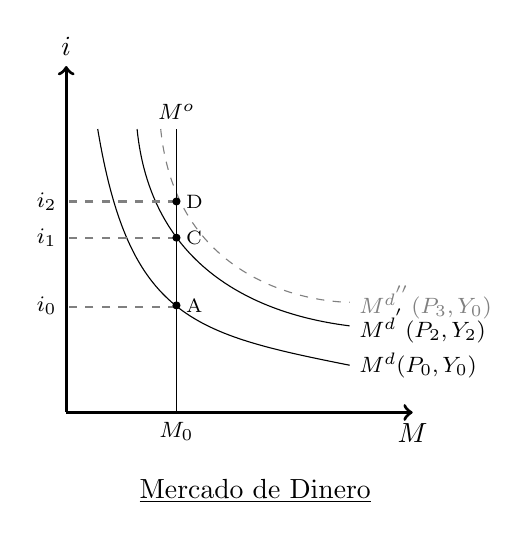
\begin{tikzpicture}[scale=0.4]
\draw[very thick,<-] (0,11) node[above]{$i$}--(0,0);
\draw[very thick,->] (0,0)--(11,0) node[below]{$M$};
\node[right] at (0,11) {};
\node[] at(6,-2.5) {\underline{Mercado de Dinero}};
\draw[thin] (1,9).. controls (2,3) and (4, 2.5) .. (9, 1.5) node [right]{\footnotesize $M^{d} (P_0, Y_0)$};
\draw[thin] (2.25,9).. controls (2.75,4) and (7, 3) .. (9, 2.75) node [right]{\footnotesize $M^{d^{'}} (P_2, Y_2)$};
\draw[thin, gray, dashed] (3,9).. controls (3.5,4) and (8, 3.5) .. (9,3.5) node [right]{\footnotesize $M^{d^{''}} (P_3, Y_0)$};
\draw[thin](3.5, 0)--(3.5, 9) node [above]{\footnotesize $M^{o}$};
\draw[thick, gray, dashed] (3.5,3.35)--(0,3.35);
\draw[thick, gray, dashed] (3.5,5.55)--(0,5.55);
\draw[thick, gray, dashed] (3.5,6.7)--(0,6.7);
\draw[fill] (3.5,3.4) circle [radius =0.11] node[right] {\scriptsize A};  
\draw[fill] (3.5,5.55) circle [radius =0.11] node[right] {\scriptsize C};  
\draw[fill] (3.5,6.7) circle [radius =0.11] node[right] {\scriptsize D}; 
\node[below] at (3.5,0) {\footnotesize $M_0$};
\node[left] at (0,3.4) {\footnotesize $i_0$};
\node[left] at (0,5.55) {\footnotesize $i_1$};
\node[left] at (0,6.7) {\footnotesize $i_2$};
\end{tikzpicture}
\end{center}
\end{minipage}
\end{center}
\end{figure}
\end{center}
\end{frame}


\begin{frame}{Expansión fiscal/deuda/no ricardianos/keynesiano}
   
\begin{itemize}
\item La reversión de la demanda agregada no es plena con lo que aumenta 
\item Pero los precios no aumentan con lo que sube el producto
\item Esto empuja para arriba la demanda de dinero y la tasa de interés nominal
\item En el mercado de crédito el gobierno aumenta la demanda, el aumento en la demanda de dinero reduce algo la oferta (compensado parcialmente por el aumento del producto) 
\item Acá el equilibrio es con un mayor nivel de crédito, no hay crowding out total porque el producto aumentó! 
\item En el mercado de trabajo los salarios no se mueven y aumenta el empleo  
\end{itemize}
\end{frame}


\begin{frame}{Discusión}

    \begin{itemize}
    \item Para un clásico hay poco por hacer: más vale concentrarte en lo estructural: competencia, apertura, instituciones
    \item En el mundo keynesiano, al menos hay margen, pero…
    \item A) La mayor parte de los cambios en el producto son generados por cambios en C e I, causados por los agentes individuales, inducidos por el ambiente político y las expectativas
    \item B) ¿Estamos seguros el gobierno será efectivo o incluso si actuará cuando debe actuar? 
    \end{itemize}

\end{frame}

%---------------------------------------------------------------------------%

\begin{frame}{Caveats a la política macroeconómica}

    \begin{itemize}
    \item Puede existir un problema de rezagos: las políticas pueden hacerse en un momento inadecuado
    \item Podes pensar que podes cuando no podes (si el mundo es clásico, las políticas sólo van a resultar en inflación o deflación)
    \item Si el marco político genera gobiernos débiles, puede existir prociclicalidad fiscal o exceso de gasto
    \item Las políticas pueden incrementar la incertidumbre
    \item La gente puede anticipar estas políticas haciéndolas menos efectivas (inconsistencia temporal y expectativas racionales), por ejemplo si vos aumentas el dinero y la gente se da cuenta al toque, los precios suben y no lográs nada
    \end{itemize}

\end{frame}
\begin{frame}{Las tipologías de la macro}
\begin{table}[]
\resizebox{\textwidth}{!}{%
\begin{tabular}{|c|c|c|}
\hline
           & Shock a la oferta                                                                      & Shock a la demanda           \\ \hline
Clasico    & Teoria del ciclo real                                                                  & Inefectividad de la politica \\ \hline
Keynesiano & \begin{tabular}[c]{@{}c@{}}Conflicto entre estabilidad\\ y estabilización\end{tabular} & Divina coincidencia          \\ \hline
\end{tabular}%
}
\end{table}

\end{frame}



\end{document}







